\section{Higher-order weak lensing statistics}
\label{sec:HOWLS}

\begin{figure*}
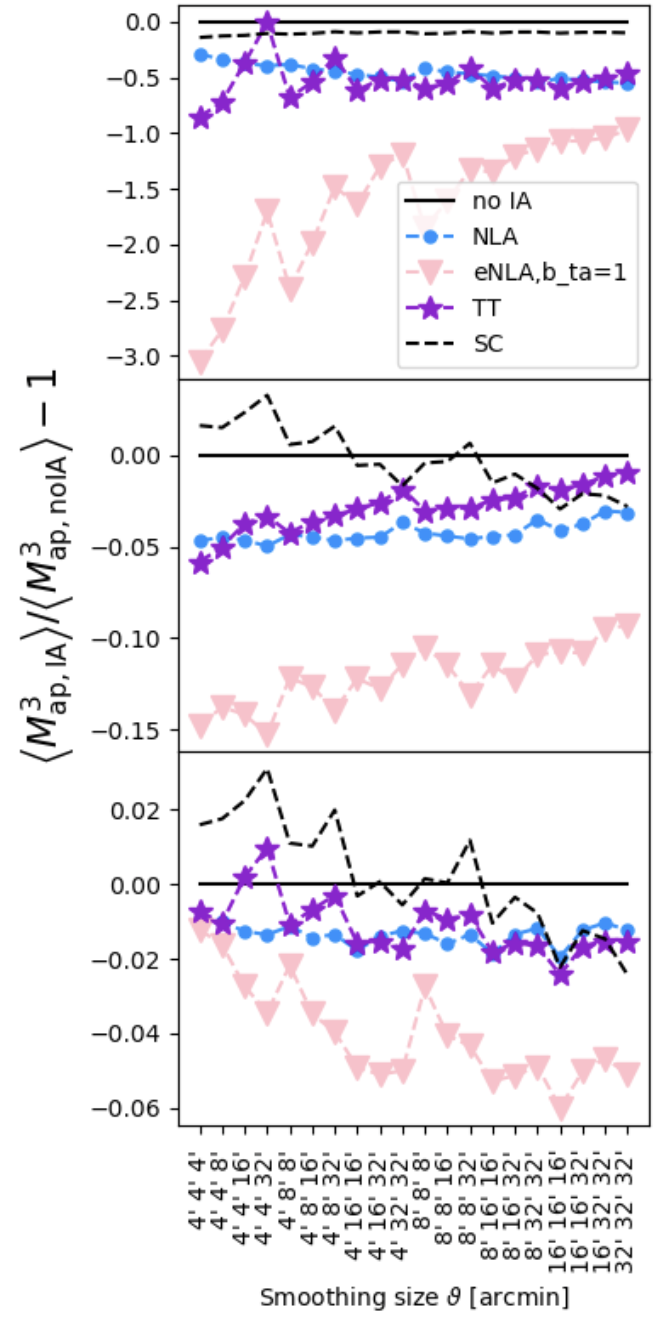
\includegraphics[width=2.7in]{graphs/Map3_IA}
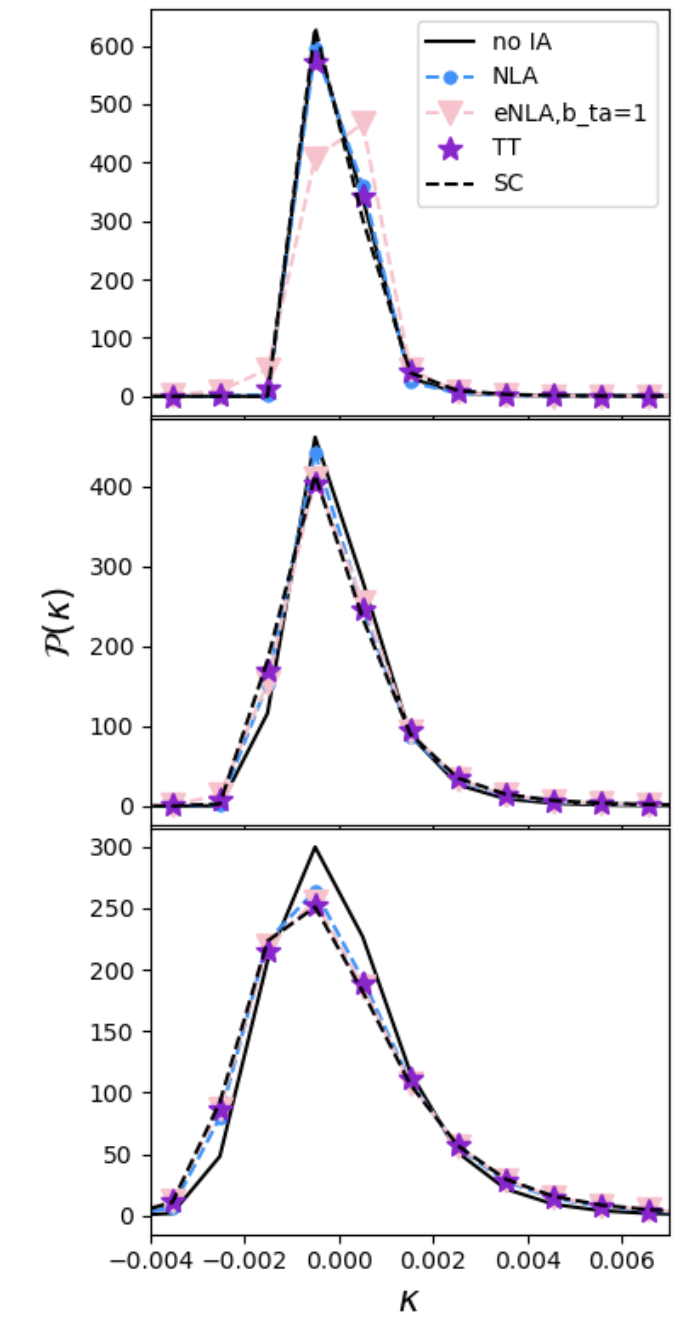
\includegraphics[width=2.7in]{graphs/PDF_IA}
\caption{Impact of IA on the $M_{\rm ap}^3$ (left) and lensing PDF (right) statistics (see Sec. \ref{subsec:beyond-2pt}), for different combinations of smoothing scales $\vartheta$ and IA models. The three panels are, from top to bottom, showing the results from tomographic bins 1 to 3, respectively. ({\it This is huge and wrong! Must redo with new maps.})}
\label{fig:Map3_IA}
\end{figure*}

\begin{figure*}
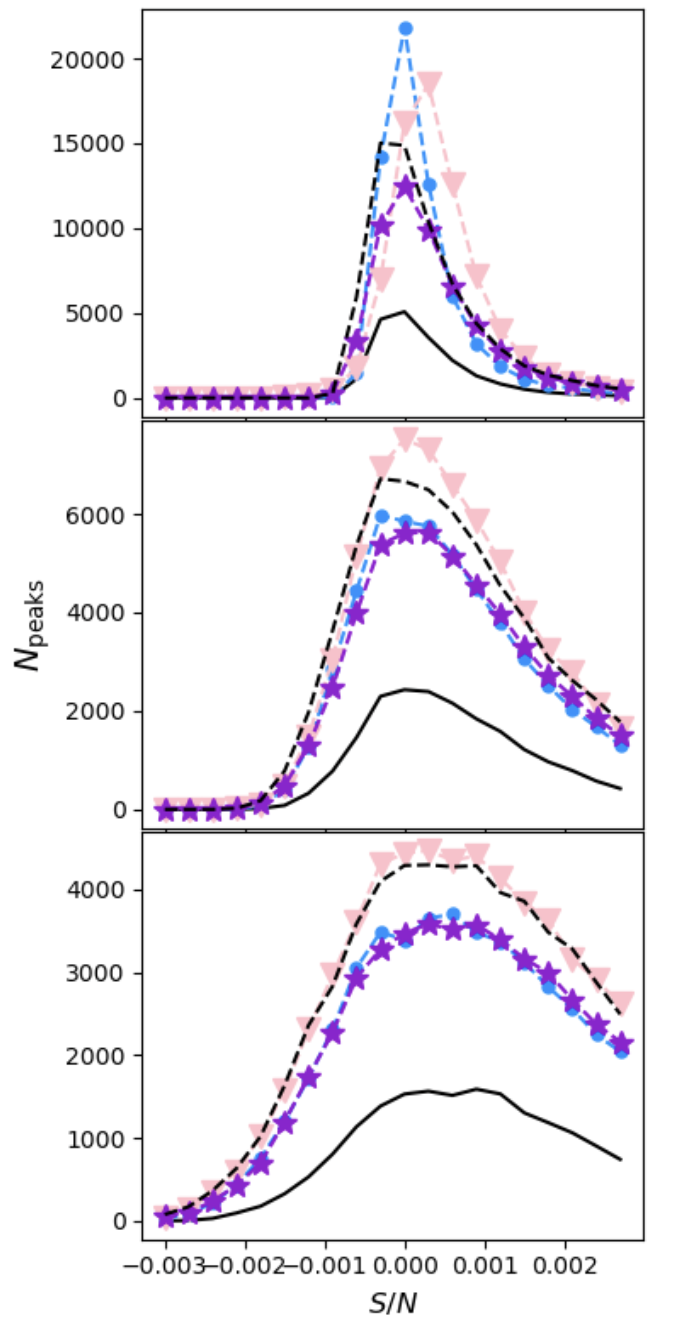
\includegraphics[width=1.65in]{graphs/Peaks_IA}
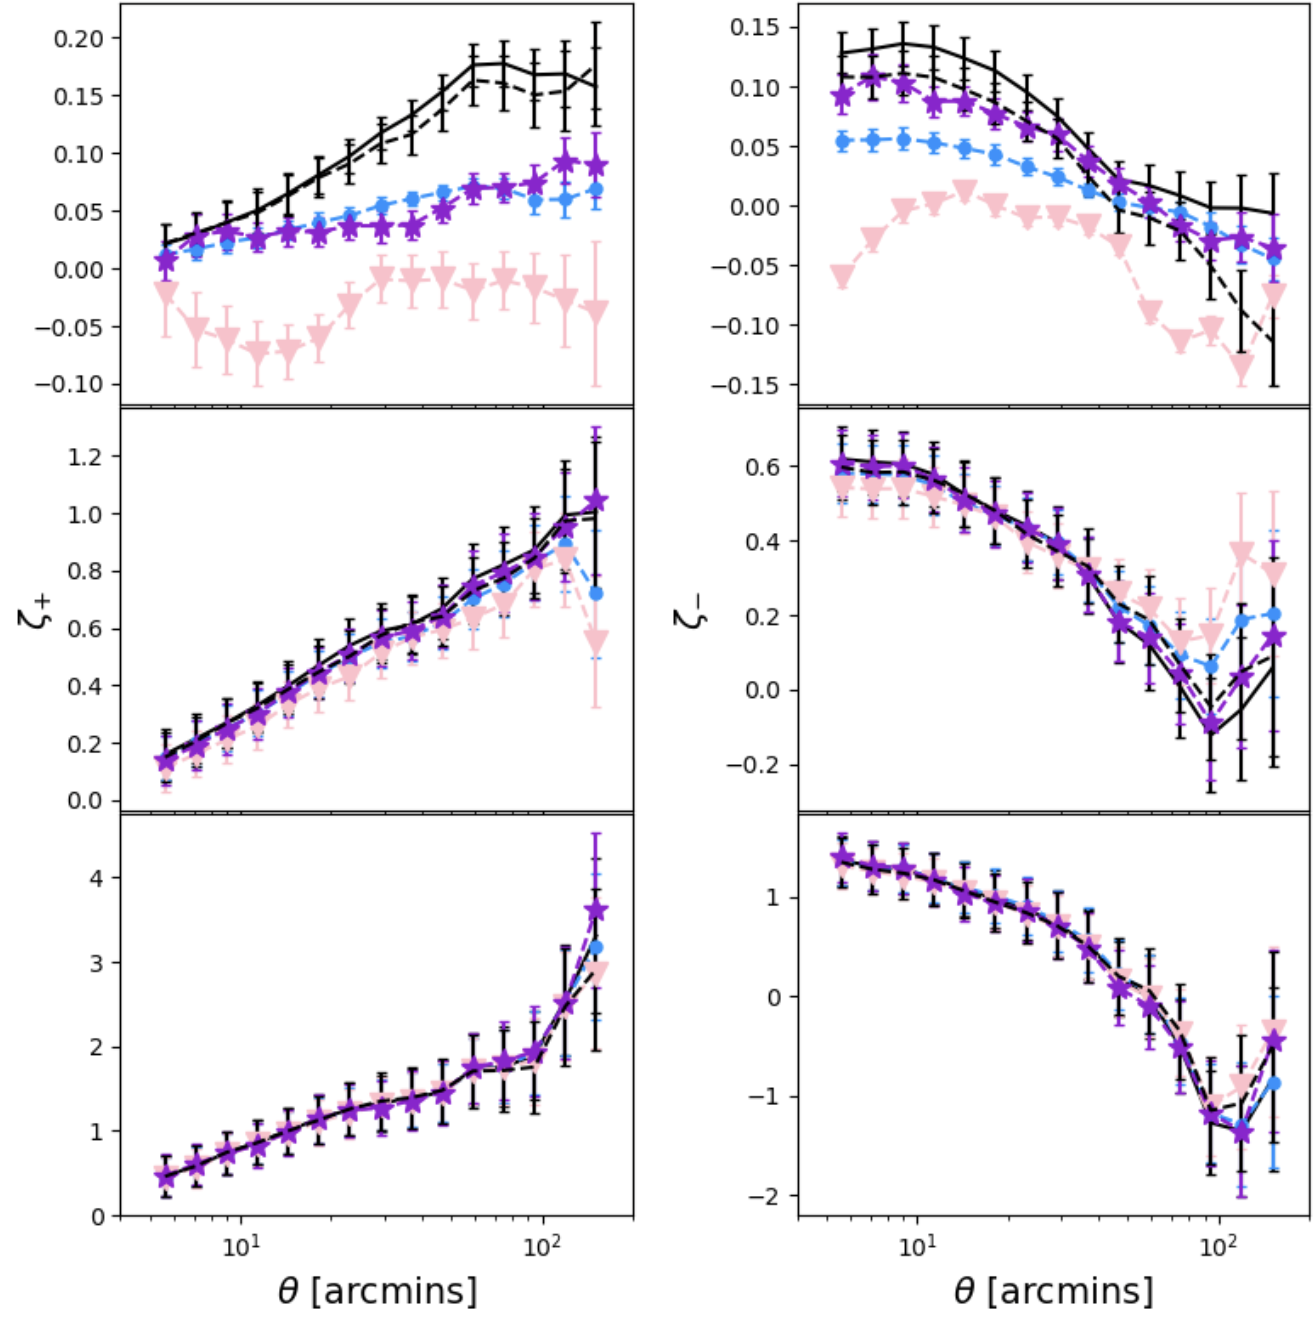
\includegraphics[width=3.3in]{graphs/i3PCF}
\caption{Impact of different IA models on the peak statistic (left) and on the integrated three-point shear statistics $\zeta_+$ (centre) and $\zeta_-$ (right).}
\label{fig:I3PCF}
\end{figure*}


This Section presents the impact of different IA model presented in Table \ref{table:IAmodels} on the measurements from higher-order weak lensing statistics introduced in Sec. \ref{subsec:beyond-2pt}. We focus on the relative impact on the data vector, but this could easily be extended to compute the derivatives with respect to the different IA parameters $[A_{\rm IA}, b_{\rm TA}, C_2]$, which can then be used in Fisher forecasts or for forward-modelling the effect directly inside  a likelihood analysis  as in e.g. \citet{DESY1_Heydenreich, KiDS1000_Burger, KiDS1000_JHD}. This method assumes that the data vector can be Taylor expanded to first order about the systematic parameters  
\begin{eqnarray}
f(A_{\rm IA},b_{\rm TA},C_2) = f({\rm no-IA}) +  \sum_p \frac{{\rm d}f}{{\rm d}p}\times p \, ,
\end{eqnarray}
with $ p=[A_{\rm IA}, b_{\rm TA}, C_2]$ and $f$ any weak lensing statistics. This is of course  neglecting higher-order correlations between parameters, or variations with cosmology, but that is often a good approximation. 

Fig. \ref{fig:Map3_IA} shows the results for the $M_{\rm ap}^3$  and lensing PDF  statistics, where we can see that the impact is the largest at low redshift. Specifically, the different models do not impact the probes at the same level. For instance, ...